\documentclass[letterpaper, 12pt, oneside, spanish]{tesis}

% Paquetes para idioma
\usepackage{babel}
\usepackage[utf8]{inputenc}

% Otros paquetes instalados
% Básicos
\usepackage[backend=bibtex,style=alphabetic]{biblatex}
\addbibresource{bibliografia.bib}
\usepackage{enumerate}
\usepackage{csquotes}
\usepackage{url}
\usepackage{datetime}
\longdate

% Para dibujar figuras
\usepackage{tikz}

% Para cambiar el color de las letras
\usepackage{color}

% Para incluir código (básico)
\usepackage{verbatim}
\usepackage{fancyvrb}

% Para incluir hipervínculos
\usepackage{hyperref}
\hypersetup{urlcolor=blue, colorlinks=false}

% Para más símbolos matemáticos
\usepackage{amsmath}
\usepackage{amsthm}
\usepackage{amssymb}

% Para colocar teoremas en cajas
\usepackage{mdframed}

% Para texto Lorem Ipsum
\usepackage{blindtext}

% Para suprimir algunas advertencias
\usepackage{silence}

\WarningFilter{blindtext}{}     % Supress the "spanish not defined, using English instead"

% Paquetes locales
% Puedes agregar paquetes locales (archivos .sty) en un subdirectorio % 'paquetes'.
% Utiliza la sintaxis \usepackage{paquetes/nombrePaquete}

% Todas las imágenes se cargan del subdirectorio 'img' por defecto.
\graphicspath{{img/}}

% Sangrías de 3 espacios (3 veces el espacio de la x)
\parindent 3ex

% Interlineado
\setlength{\baselineskip}{1.5pt}

% Interpárrafo
\setlength{\parskip}{16.5pt}

\topmargin 2cm

\renewcommand{\tablename}{Tabla}
\newcommand\listsymbolname{Acrónimos y Símbolos}

% Para colocar un margen a la izquierda
\newmdenv[
        hidealllines=true,
        leftline=true,topline=true,
        frametitleaboveskip=-5pt,
        linewidth=1.5pt,
    ]{leftframe}

\newenvironment{coloredframe}[2]{
    \mdfsetup{frametitle={\colorbox{white}{\space#1\space}},linecolor=#2}
    \begin{leftframe}
}{
    \end{leftframe}
}

% greens
\definecolor{caribbeangreen}{rgb}{0.0, 0.8, 0.6}

% blues
\definecolor{cerulean}{rgb}{0.0, 0.48, 0.65}
\definecolor{cyan process}{rgb}{0.0, 0.72, 0.92}

% reds
\definecolor{crimson}{rgb}{0.86, 0.08, 0.24}
\definecolor{darkcandyapplered}{rgb}{0.64, 0.0, 0.0}

\lstdefinelanguage{angler}{
    % add these letters as possible parts of keywords
    alsoletter={:, \\, =, -, >, \_, ., (, ), \{, \}},
    % list of keywords
    morekeywords={
        export, import, as, open, reopen, closed, with,
        where, let, in,
        forall, exists, select,
        behaviour, on, defines, is,
        operator, prefix, postfix, infixL, infixR, infixN
    },
    % symbol keywords
    morekeywords={
        [2]:, [2]=, [2]\\, [2]->, [2].,
        [2]\_, [2](, [2]), [2]\{, [2]\}
    },
    sensitive=true,                 % keywords are case-sensitive
    morecomment=[l]{\-\-},          % line comments
    morecomment=[s]{\{\-}{\-\}},    % block comments
    morestring=[b]",                % strings are in double quotes
    morestring=[d]',                % characters are in single quotes
}

\newcommand{\inlinemath}[1]{{\small\bfseries\color{cyan process}\texttt{$#1$}}}
\newcommand{\inlinecode}[1]{{\small\bfseries\color{darkcandyapplered}\texttt{#1}}}
\lstnewenvironment{anglercode}[1][]{
    \linespread{1}
    \lstset{
        language=angler,
        keywordstyle={\color{cerulean}\bfseries},   % style for keywords: bold
        keywordstyle={[2]\bfseries},
        commentstyle={\color{gray}},        % style for comments
        captionpos=t,                       % caption position: top
        frame=lt,                           % frame: left and top
        frameround=ffff,                    % roundness: TR, BR, BL, TL
        framerule=0.75pt,                   % thickness of the frame
        framesep=0.5cm,                     % separation from frame to code
        rulecolor=\color{gray},
        columns=flexible,                   % flexible character width
        keepspaces=true,                    % keep all spaces
        % margins
        aboveskip=1cm, xleftmargin=1.25cm, xrightmargin=1.25cm,
        % listings does not support UTF-8
        literate= {á}{{\'a}}1 {é}{{\'e}}1 {í}{{\'i}}1 {ó}{{\'o}}1 {ú}{{\'u}}1
                  {Á}{{\'A}}1 {É}{{\'E}}1 {Í}{{\'I}}1 {Ó}{{\'O}}1 {Ú}{{\'U}}1
                  {à}{{\`a}}1 {è}{{\`e}}1 {ì}{{\`i}}1 {ò}{{\`o}}1 {ù}{{\`u}}1
                  {À}{{\`A}}1 {È}{{\'E}}1 {Ì}{{\`I}}1 {Ò}{{\`O}}1 {Ù}{{\`U}}1
                  {ä}{{\"a}}1 {ë}{{\"e}}1 {ï}{{\"i}}1 {ö}{{\"o}}1 {ü}{{\"u}}1
                  {Ä}{{\"A}}1 {Ë}{{\"E}}1 {Ï}{{\"I}}1 {Ö}{{\"O}}1 {Ü}{{\"U}}1
                  {â}{{\^a}}1 {ê}{{\^e}}1 {î}{{\^i}}1 {ô}{{\^o}}1 {û}{{\^u}}1
                  {Â}{{\^A}}1 {Ê}{{\^E}}1 {Î}{{\^I}}1 {Ô}{{\^O}}1 {Û}{{\^U}}1
                  {œ}{{\oe}}1 {Œ}{{\OE}}1 {æ}{{\ae}}1 {Æ}{{\AE}}1 {ß}{{\ss}}1
                  {ű}{{\H{u}}}1 {Ű}{{\H{U}}}1 {ő}{{\H{o}}}1 {Ő}{{\H{O}}}1
                  {ç}{{\c c}}1 {Ç}{{\c C}}1 {ø}{{\o}}1 {å}{{\r a}}1 {Å}{{\r A}}1
                  {€}{{\EUR}}1 {£}{{\pounds}}1 {¿}{{\textquestiondown}}1
                  {¡}{{\textexclamdown}}1,
        #1                                  % settings for the lst environment
    }
}{}

% Macros
\newcommand{\projectTitle}{Angler}
\newcommand{\authorName}{Matteo José Ferrando Briceño}
\newcommand{\tutorName}{Ricardo Monascal}

\newdate{presentationdate}{16}{3}{2016}

\begin{titlepage}
    \title{
        \vspace{-2cm} 
\includegraphics[width=1.2in]{./usb.png} \\[.2cm]
        \large Universidad Simón Bolívar \\
        Decanato de Estudios Profesionales \\
        Coordinación de Ingeniería de la Computación
        \vfill \LARGE \projectTitle \vfill
    }
    \author{Por: \\
        \authorName \\[1.2cm]
        Realizado con la asesoría de: \\
        \tutorName \\[1.2cm]
        PROYECTO DE GRADO \\
        Presentado ante la Ilustre Universidad Simón Bolívar \\
        como requisito parcial para optar al título de \\
        Ingeniero de Computación
    }
    \date{Sartenejas, \monthname[\the\month] de \the\year}
\end{titlepage}

\begin{document}
\frontmatter
\maketitle
\setstretch{1.3}

% Se incluye el acta de evaluación, verificar que se corresponda
% con el formato aceptado actualmente por el Decanato.
% Pagina del acta final
\begin{titlepage}
\begin{center}

% Upper part

\includegraphics[scale=0.5]{usb.png} \\

\textsc {\large UNIVERSIDAD SIMÓN BOLÍVAR} \\
\textsc{DECANATO DE ESTUDIOS PROFESIONALES\\
COORDINACIÓN DE INGENIERÍA DE LA COMPUTACIÓN}

\bigskip
\bigskip
\bigskip
\bigskip
\bigskip
\bigskip

% Title
\textsc{ACTA FINAL PROYECTO DE GRADO}

\bigskip
\bigskip

\textsc{\textbf{\projectTitle}}

\bigskip
\bigskip
\bigskip
\bigskip

\begin{minipage}{\textwidth}
\centering
Presentado por: \\
\textsc{\textbf{\authorName}} \\

\bigskip
\bigskip
\bigskip

Este Proyecto de Grado ha sido aprobado por el siguiente jurado examinador: \\

\bigskip
\bigskip

{   % for \juryinfo to only exist here
\newcommand{\juryinfo}[1]{
\line(1,0){200} \\
#1 \\

\bigskip
\bigskip
}

% Despues de cada line coloca el (los) nombre(s) de
% cada uno de los integrantes del jurado.
\juryinfo{\tutorName}
\juryinfo{@jurado1}
\juryinfo{@jurado2}
}

\end{minipage}
\vfill

% Date/Fecha
{\large \bfseries Sartenejas, \displaydate{presentationdate}}

\end{center}
\end{titlepage}


% El resumen debe ser de una sola página
\addtotoc{Resumen}
\abstract{
\addtocontents{toc}{\vspace{1em}}
\blindtext

% Las palabras clave son generalmente los nombres de áreas de investigación a
% los cuales está asociado el trabajo. Generalmente son tres o cuatro.
\noindent \begin{small} \textbf{Palabras clave}: @palabra1, @palabra2, @palabra3.
\end{small}
}

% Iniciar nueva página luego del resumen
\clearpage
\setstretch{1.3}

% Agradecimientos
\acknowledgements{
\addtocontents{toc}{\vspace{1em}}
\blindtext
}
\clearpage

\pagestyle{fancy}

% Tabla de contenidos o índice
\lhead{\emph{Índice General}}
\tableofcontents

% Estos índices solamente se usan si el libro contiene figuras, tablas y
% algoritmos. Si alguno de estos no se utiliza, comentar o eliminar las líneas
% pertinentes.
\lhead{\emph{Índice de Figuras}}
\listoffigures

\lhead{\emph{Índice de Tablas}}
\renewcommand*\listtablename{Índice de Tablas}
\listoftables

%\lhead{\emph{Índice de Algoritmos}}
%\renewcommand*\listalgorithmname{Índice de algoritmos}
%\listofalgorithms

\setstretch{1.5}
\clearpage
\lhead{\emph{Acrónimos y símbolos}}
\listofsymbols{ll}
{

    % Aquí van las siglas
    \textbf{SIGLAS} & \textbf{S}iglas \textbf{I}sla \textbf{G}rafo
                      \textbf{L}aos \textbf{A}ve \textbf{S}erpiente\\
    \textbf{ACM} & \textbf{A}ssociation for \textbf{C}omputing \textbf{M}achinery\\
    &\\
    \hline
    &\\

    % Aquí van los símbolos
    $\iff$ & doble implicación, si y sólo si\\
    $\Rightarrow$ & implicación lógica\\
    $[u:=v]$ & sustitución textual de $u$ por $v$
}

%% ----------------------------------------------------------------
% End of the pre-able, contents and lists of things
% Begin the Dedication page

\setstretch{1.3}  % Return the line spacing back to 1.3

\pagestyle{empty}  % Page style needs to be empty for this page

\dedicatory{
    \textbf{Dedicatoria} \bigskip

    A @personasImportantes, por @razonesDedicatoria.
}

\addtocontents{toc}{\vspace{2em}}

\mainmatter
\pagestyle{fancy}

% Se incluye el cuerpo de la tesis en este documento.

\chapter*{Introducción}
\label{intro}
\lhead{\emph{Introducción}}
\addcontentsline{toc}{chapter}{Introducción}

% Descripción del problema, de lo general hacia lo específico
\blindtext

% Trabajos anteriores
\blindtext

En \cite{article:mixfix} se presenta un trabajo que \ldots

% \citeauthor{article:mixfix} es otro autor que \ldots

% Objetivo general
\blindtext

% Objetivos específicos
\blinditemize

Cachucha\footnote{Lorem Ipsum.}.

% Organización del trabajo
% Se describe brevemente qué se hace en cada capítulo
\blindtext[4]


% El número de capítulos varía. En mi libro fueron cuatro (sin contar
% introducción y conclusión).
\chapter{@nombreCapítulo}
\label{capitulo1}
\lhead{Capítulo 1. \emph{@nombreCapítulo}}

% De qué va a tratar el capítulo
% El capítulo 1 suele ser el marco teórico.

\section{@sección}
\begin{definition}
\label{definicion1}
\blindtext, donde:
\begin{itemize} 
\item $X$ es $\gamma - 2$.
\item $A$ es un conjunto de \textbf{cosas}.
\end{itemize}
\end{definition}

La Figura \ref{usb} muestra el símbolo de nuestra universidad.
\begin{figure}[h!]
\centering

\includegraphics[width=0.4\textwidth]{usb.png}
\caption[La popular \textit{cebolla}]{La popular \textit{cebolla}, símbolo de la USB.}
\label{usb}
\end{figure}

\begin{verbatim}
para escribir código
    básico
\end{verbatim}
\Blindtext

\begin{Verbatim}[commandchars=\\\{\}, codes={\catcode`$=3\catcode`^=7}]
var x = 21;
if (esto_es_código) {
    imprimir(foo);
}
(lisp (listas (?paréntesis))
\end{Verbatim}

\blindtext
\subsection{@subSección}
\Blindtext

\section{@sección}
\blindtext

\begin{mdframed}
\begin{theorem}
\label{principal}
\textbf{Propiedades formales}
\blindenumerate
\end{theorem}
\end{mdframed}

\subsection{@subsección}
\subsubsection{@subsubsección}
\blindenumerate

La Figura \ref{grafo} lo muestra.

\shorthandoff{<>."}
\begin{figure}[h]
\begin{center}
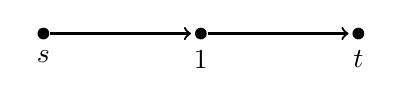
\begin{tikzpicture}[shorten >=1pt, thick]%[shorten >=1pt,node distance=2cm,>=stealth',thick]
  \node [shape=circle,fill=black,inner sep=1.5pt,label=below:$s$] (q0) at (0,0) {};
  \node [shape=circle,fill=black,inner sep=1.5pt,label=below:$1$] (q1) at (2,0) {};
  \node [shape=circle,fill=black,inner sep=1.5pt,label=below:$t$] (q2) at (4,0) {};
  \path[->] (q0) edge (q1) (q1) edge (q2);
\end{tikzpicture}
\end{center}
\caption[@descripcionCorta]{@descripcionLarga}
\label{grafo}
\end{figure}

\begin{enumerate}[--]
\item 1
\item 2
\item 3
\end{enumerate}

\begin{tabular}{ll}
1 & 2\\ \hline
1 & 2\\
1 & 2\\
\end{tabular}

\blindtext. Tabla \ref{tabla:resultados}.

\begin{figure}[h]
\begin{alignat*}{1}
A\   & \longrightarrow B \mid C\\
\end{alignat*}
\caption[Gramática]{Gramática de un lenguaje.}
\label{gram}
\end{figure}

\blindtext
\begin{table}[h!]
\begin{center}
\begin{tabular}{llllll}
\multicolumn{4}{@{}c}{Nombre del experimento} \\
\midrule
              &    éxitos/intentos & tiempo (ms) & espacio (kB) \\
\midrule
instancia1          &        28/30 &    23 &       1.7 \\
instancia2          &        50/70 &    12 &       32.7 \\
\midrule
\end{tabular}
\end{center}
\caption[Resultados X/Y]{Resultados de X para Y}
\label{tabla:resultados}
\end{table}

\begin{equation}
\label{eq}
\Phi = (\forall x) (R x)
\end{equation}

En el Apéndice \ref{apendiceA} se encuentra.

% \def\chapterTitle{Marco Tecnológico\xspace}

\chapter{\chapterTitle}
\label{capitulo2}
\lhead{Capítulo 2. \emph{\chapterTitle}}

\Blindtext

% \def\chapterTitle{Marco Metodológico\xspace}

\chapter{\chapterTitle}
\label{capitulo3}
\lhead{Capítulo 3. \emph{\chapterTitle}}

\Blindtext

\def\chapterTitle{Desarrollo\xspace}

\chapter{\chapterTitle}
\label{ch:development}
\lhead{Capítulo 4. \emph{\chapterTitle}}

\newenvironment{investigationfr}
    {\begin{leftframe}[frametitle={Investigación},linecolor=caribbeangreen]}
    {\end{leftframe}}
\newenvironment{designfr}
    {\begin{leftframe}[frametitle={Diseño},linecolor=cerulean]}
    {\end{leftframe}}
\newenvironment{implementationfr}
    {\begin{leftframe}[frametitle={Implementación},linecolor=crimson]}
    {\end{leftframe}}

\begin{investigationfr}
\end{investigationfr}

\begin{designfr}
\end{designfr}

\begin{implementationfr}
\end{implementationfr}

\section{Ideas iniciales}

\begin{designfr}
Se comenzó con algunas ideas que consideramos básicas para el lenguaje.

\begin{itemize}
    \item El lenguaje debe ser explícito, es decir, no se deben inferir las ideas presentadas en un programa.
    \item La definición del lenguaje debe ser compacta.
    \item El lenguaje debe ser amistoso para principiantes.
    \item El sistema de tipos debe tener tipos dependientes.
    \item Los alcances del lenguaje deben ser determinados por la indentación.
\end{itemize}
\end{designfr}

\section{Expresiones, tipos y sus constructores}

\begin{designfr}
Ya que el lenguaje debe tener tipos dependientes, se decidió desde un principio que un tipo es sencillamente una expresión, no un elemento especial del lenguaje, hace que en cualquier parte donde se espera un tipo, debería poder escribirse cualquier expresión, mientras que el chequeo de tipos pase sin errores.

Al hacer estos dos elementos uno solo, se definieron las diferentes construcciones posibles de expresiones.

\begin{itemize}
    \item Aplicación de funciones
    \item Parentización
    \item Lambda funciones
    \item Pattern matching
    \item Alcance de declaraciones para una expresión (\inlinecode{where}, \inlinecode{let-in})
    \item Cuantificadores universales y existenciales de tipos
\end{itemize}
\end{designfr}

\section{Tipos y funciones, ¿abiertos o cerrados?}

\begin{designfr}
Nos preguntamos porqué se ha hecho una diferencia tan clara en otros lenguajes de programación funcionales entre lo que es una función, un tipo y un constructor de tipo, así que comenzamos con la idea de que todos éstos fueran declarados de la misma manera.

\begin{anglercode}
Bool : Type
True : Bool
False : Bool

not : Bool -> Bool
not True = False
not False = True
\end{anglercode}

Esta alternativa hacía que la única diferencia entre una función y un tipo es que no tenga declaraciones asociadas, pero el siguiente ejemplo nos dejó preguntándonos qué debería suceder:

\begin{anglercode}
Bool : Type
True : Bool
False : Bool

not : Bool -> Bool
not True = False
not False = True

True = False    -- ¿los pattern matching ahora son inválidos?
\end{anglercode}

¿Ahora \inlinecode{True} deja de ser algo sobre lo que se puede hacer pattern matching, como en la función \inlinecode{not}?; como podemos ver, da paso a que un programa deje de funcionar con tan solo una línea sospechosa.

Otro ejemplo que da paso a problemas sería agregar un constructor a un tipo que no se debe:

\begin{anglercode}
Bool : Type
True : Bool
False : Bool

not : Bool -> Bool
not True = False
not False = True

IDK : Bool

not IDK         -- ¿qué debería reportarse aquí?
\end{anglercode}

Aquí agregamos un nuevo constructor a el tipo \inlinecode{Bool} y aunque tenga sentido usarlo en la función \inlinecode{not}, pues espera algo del tipo \inlinecode{Bool}, el programa va a dar un error al correr, no al ser analizado por errores estáticos.

Así que se nos ocurrieron los tipos cerrados, éstos son tipos cuyos constructores son listados inmediatamente en un alcance nuevo, y no se le puede agregar más constructores.

\begin{anglercode}
Bool : Type where
    True : Bool
    False : Bool

not : Bool -> Bool
not True = False
not False = True
\end{anglercode}

Y ahora ninguno de las confusiones anteriores suedería, al declarar el \inlinecode{IDK} no habría problema, pero al llamar \inlinecode{not IDK}, el intepretador reportaría un error estático.

Luego al ver \inlinecode{where} puede ser utilizado al final de cualquier expresión, por lo que no era una palabra que pudieramos utilizar para introducir los constructores, así que optamos por la palabra \inlinecode{with}. También el cambio muestra la diferencia semántica entre \inlinecode{where} y \inlinecode{with}, con el \inlinecode{where} se introduce un alcance sólo disponible en la expresión de éste, mientras que el \inlinecode{with} introduce elementos en el alcance exterior a éste.

\begin{anglercode}
Bool : t where t = Type
    with
        True : Bool
        False : Bool
\end{anglercode}

Pero parecía interensante la idea de tipos que sus constructores pudieran ser agregados mientras se fueran necesitando, viene en mente un ejemplo de monedas del mundo con tan solo algunas monedas \textit{base}, para que el usuario agregue las de interés.

\begin{anglercode}
Currency : Type
USD : Nat -> Currency
EUR : Nat -> Currency

toUSD : Currency -> Currency
toUSD (USD n) = USD n
toUSD (EUR n) = USD (n * 1.1)

-- ...

XBT : Nat -> Currency   -- bitcoin
toUSD (XBT n) = USD (n * 400)
\end{anglercode}

Así que si tenemos tipos abiertos y cerrados, tendremos también funciones abiertas y cerradas; ya que estamos buscando enlazar lo más posible estos dos conceptos:

\begin{anglercode}
not : Bool -> Bool where
    not True = False
    not False = True
\end{anglercode}

Pero los tipos abiertos seguían sufriendo de los problemas presentados al principio, habría que hacer una diferencia más explícita entre tipos y funciones.

Los tipos, abiertos y cerrados, deben indicar explícitamente cuáles son sus constructores de tipos para evitar el problema antes mencionado, de forma que llegamos a la siguiente sintaxis:

\begin{anglercode}
closed Bool : Type with
    True : Bool
    False : Bool

not : Bool -> Bool
not True = False
not False = True

closed Nat : Type with
    Z : Nat             -- cero
    S : Nat -> Nat      -- sucesor

open Currency : Type with
    USD : Nat -> Currency
    EUR : Nat -> Currency

toUSD : Currency -> Currency
toUSD (USD n) = USD n
toUSD (EUR n) = USD (n * 1.1)

-- ...

reopen Currency with
    XBT : Nat -> Currency

toUSD (XBT n) = USD (n * 400)
\end{anglercode}

Además todo este análisis nos hizo darnos cuenta de que aunque los tipos, constructores de tipos y funciones compartan muchas cualidades, no son lo mismo, se diferencian semánticamente y ésto debería mostrarse en su definición también.

Haciendo finalmente claras las diferencias, dejamos de un lado la idea de funciones cerradas; aunque éstas pueden ser teóricamente interesantes, no conseguimos gran utilidad práctica, ya que de querer \textit{cerrar} una función abierta, simplemente se deben escribir todos los casos posibles de sus argumentos.

\begin{anglercode}
isUSD : Currency -> Bool
isUSD (USD _) = True
isUSD _ = False         -- *cierra* la función

-- ...

isUSD (XBT _) = True    -- este caso nunca correrá
\end{anglercode}
\end{designfr}

\section{Identificadores, ¿mayúscuas o minúsculas?}

\begin{designfr}
En un principio se consideró usar la convención de Haskell, que los constructores de tipos y tipos se escribieran con la primera letra mayúscula, y que los valores con la primera letra minúscula; de esta manera se podía distinguir sintácticamente entre ellos.

Pero esta idea tenía algunos problemas, por ejemplo, los identificadores que comenzaran con símbolos y no letras, ¿a qué clase pertenecerían?, además debemos recordar que con tipos dependientes, los tipos son expresiones como cualquier otra, por lo que una distinción sintáctica entre el \emph{uso} de tipos y valores no era conveniente.
\end{designfr}

\section{Cuantificadores: parámetros y argumentos implícitos}

\begin{designfr}
Como se busca un lenguaje explícito, todo identificador que se utilice en una expresión, debe estar previamente definido con un tipo acompañante, tomando inspiración de otros lenguajes con tipos dependientes llegamos a la idea de tener dos secciones de la firma de una función, la parte \emph{implícita}, que es el cuantificador universal; y la parte \emph{explícita}:

\begin{anglercode}
compose : { (a:Type) -> (b:Type) -> (c:Type) } -> (b -> c) -> (a -> b) -> a -> c
\end{anglercode}

Donde se escribe la parte implícita entre llaves (\inlinecode{\{} y \inlinecode{\}}) como un tipo más, y luego se escribe la parte explícita, donde todos los nombres introducidos en la parte implícita están disponibles. Esto nos dejaba con dudas acerca de cómo se podían escribir con una estructura similar los tipos existenciales.

Los argumentos implícitos se pasan a la función al comenzar su nombre con un caracter \emph{piso} (\inlinecode{\_}):

\begin{anglercode}
compose _Bool : { (b : Type) -> (c : Type) } -> (b -> c) -> (Bool -> b) -> Bool -> c
\end{anglercode}

Con esta sintaxis los parámetros implícitos son \emph{posicionales}, es decir, se pasan los argumentos con un orden específico. Esta manera de pasar argumentos implícitos nos da una restricción en los identificadores que se puedene escribir en el lenguaje, ya que ninguno podría comenzar con piso para poder diferenciarlos de argumentos implícitos.

Pero hay un mayor problema con la propuesta anterior, recordemos que en la teoría de tipos dependientes tenemos cuantificadores universales y existenciales; en un cuantificador universal no importa el orden de las variables declaradas, se puede especificar un valor para cualquera de las variables disponibles, es decir, los parámetros implícitos deberían ser todos accesibles para el pasaje de argumentos implícitos. Así llegamos a otra propuesta que separa completamente la sintaxis de firmas y de cuantificadores:

\begin{anglercode}
compose : { a:Type, b:Type, c:Type } (b -> c) -> (a -> b) -> a -> c
\end{anglercode}

Con esta nueva sintaxis podemos pasar argumentos implícitos en el orden que sea necesario:

\begin{anglercode}
compose { b = Nat, c = Bool } : { a:Type } (Nat -> Bool) -> (a -> Nat) -> a -> Bool
\end{anglercode}

Con esta nueva los parámetros implícitos son \emph{nombrados}, es decir, se pasan los argumentos en el orden que nos convenga, sin importar su posición, y los parámetros explícitos se mantienen posicionales.

Finalemente decidimos hacer un último cambio a esta sintaxis para hacer obvio que se trata de un cuantificador:

\begin{anglercode}
compose : forall a:Type, b:Type, c:Type . (b -> c) -> (a -> b) -> a -> c
\end{anglercode}

Ahora la definición se asemeja mucho más a un cuantificador, haciendo más explícito su uso, y además podemos acceder a todas las variables declaradas y especificarlas.

Se consideró usar la palabra \inlinecode{product} en vez de \inlinecode{forall}, pero se decidió ir por una referencia directa a lógica simbólica, aunque estos se consideren los tipos producto. De igual forma, se definen los tipos existenciales con la palabra \inlinecode{exists}, aunque se consideró la palabra \inlinecode{sum}:

\begin{anglercode}
vfilter : forall t:Type, n:Nat . (t -> Bool) -> Vect n t -> exists m:Nat . Vect m t
\end{anglercode}

Logrando una estructura parecida entre los cuantificadores universales y existenciales. El cuantificador existencial \emph{no} puede recibir argumentos implícitos. Esta sintaxis es \emph{azúcar sintáctica} para los cuantificadores existenciales, ya que estos están definidos en el lenguaje.
\end{designfr}

\section{El \emph{cuantificador} de selección}

\begin{designfr}
Luego nos dimos cuenta de que podemos querer introducir nombres para parámetros explícitos, es decir, lo que normalmente haríamos con un cuantificador universal, pero en vez de ser \emph{para todo} que sea para el valor dado. Esta idea se maneja en los lenguajes estudiados colocando una asociación de nombre directamente:

\begin{anglercode}
id' : (t : Type) -> t -> t
id' _ x = x
\end{anglercode}

Se entiende, pero nos pareció poco intuitivo, así que preferimos agregarle la palabra \inlinecode{select} para hacer obvio que se acerca al funcionamiento de los cuantificadores.

Además se lee \emph{\guillemotleft selecciona un \inlinecode{Type}, que llamaremos \inlinecode{t}\guillemotright}.
\end{designfr}

\section{Identificadores: evitando confusiones}

\begin{designfr}
Desde un principio se aceptó la idea de poder usar símbolos en los identificadores como \inlinecode{+}, \inlinecode{*} y demás, pero para facilitar el uso del lenguaje, se decidió que tendríamos dos categorías de caracteres, una para símbolos y otra para letras. De manera que ciertos caracteres, a pesar de estar juntos, se tomarían como identificadores separados:

\begin{anglercode}
var         -- var
v0          -- v0
0v0         -- 0 v0
++          -- ++
var++v0     -- var ++ v0
\end{anglercode}
\end{designfr}

\section{No me importa, te lo digo en inglés, I \emph{don't care}}

\begin{designfr}
En una función puede haber casos en que un argumento no es importante para su valor resultante, a estos argumentos se les puede asignar un nombre que no usaremos, o indicar explícitamente que no es importante.

\begin{anglercode}
const : forall t:Type, v:Type . t -> v -> t
const x ? = x
\end{anglercode}

Donde el caracter \inlinecode{?} indica que no importa ese valor, luego se decidió cambiar este caracter a \inlinecode{\_}, ya que el signo de interrogación puede transmitir la idea de que \emph{no sabemos} qué será el argumento, cuando lo que se quiere transmitir es que \emph{no importa}. Se eligió \inlinecode{\_} porque es el caracter típicamente usado por otros lenguajes para lo miso, y visualmente, al llamar tan poco la atención transmite su poca importancia.

\begin{anglercode}
const : forall t:Type, v:Type . t -> v -> t
const x _ = x
\end{anglercode}
\end{designfr}

\section{¿Identificador o caracter?}

\begin{designfr}
Los caracteres literales suelen escribirse usando comillas simples (\inlinecode{'}), así que se decidió que ningún identificador puede empezar con una comilla simple, ya que se estaría esperando un caracter literal. Comilla simple es el único \emph{símbolo} que está en ambas categorías de identificadores, la de símbolos y la de letras.

\begin{anglercode}
'a'     -- caracter
a''     -- identificador
+''     -- identificador
\end{anglercode}
\end{designfr}

\section{Operadores ahuecados}

\begin{designfr}
Un lenguaje didáctico sin operadores puede hacer curva de aprendizaje muy \emph{empinada}, por lo que la posibilidad de definir operadores es escencial. Se propuso usar \emph{operadores mixfijos}, estos funcionan para definir las \emph{partes} de un operador y sus \emph{huecos}, que es donde irían sus operandos; para indicar los huecos de un operador, usaremos el caracter piso (\inlinecode{\_}).

\begin{anglercode}
if_then_else_ : forall t:Type . Bool -> t -> t -> t
if True  then x else _ = x
if False then _ else y = y
\end{anglercode}

Esto nos crea una restricción sobre los identificadores, estos no pueden contener dos \inlinecode{\_} seguidos, ya que no sabríamos dónde termina un argumento y comienza el siguiente.

Un identificador con \inlinecode{\_} puede usarse como operador, colocando los argumentos en los huecos, o como una función normal escribiendo el identificador con los \inlinecode{\_} incluidos.

\begin{anglercode}
if_then_else_ : forall t:Type . Bool -> t -> t -> t
if_then_else_ True  x _ = x
if_then_else_ False _ y = y
\end{anglercode}

Nótese que se usa \inlinecode{\_} tanto para \emph{don't care} como para los huecos de los identificadores, e.g. \inlinecode{if\_then\_else\_\ False\ \_\ y}.
\end{designfr}

\section{Huecos entre identificadores}

\begin{designfr}
Gracias a la nueva sintaxis para operadores, se decidió que un las partes distintas de un identificador podrían ser de distintas categorías, es decir, pudiendo mezclarlas sólo cuando hay un \inlinecode{\_} de por medio.

\begin{anglercode}
if_?_:_ : forall t:Type . Bool -> t -> t -> t
if True  ? x : _ = x
if False ? _ : y = y
\end{anglercode}
\end{designfr}

\section{Definición de operadores}

\begin{designfr}
En un principio se consideró que si un identificador tiene \inlinecode{\_} se consideraría automáticamente un operador y tendría una precedencia y asociatividad por defecto, pero decidimos abandonar esa idea, pues podría generar comportamientos inesperados por usuarios. Así que llegamos a una definición para estos, donde no importa si el identificador es de una función o no, o está definido o no. Lo que se expresa es una regla de \emph{reordenamiento} de identificadores.

\begin{anglercode}
operator |_|                closed
operator if_then_else_      prefix  0
operator _==_               infixN  2
operator _+_                infixL  4
operator _-_                infixL  4
operator _*_                infixL  5
operator _/_                infixL  5
operator _^_                infixR  6
operator -_                 prefix  7
operator _!                 postfix 8

-- ...

if | a * b + c - d | == e then f ! else - f
-- if_then_else_ (_==_ (|_| (_-_ (_+_ (_*_ a b) c) d)) e) (_! f) (-_ f)
\end{anglercode}
\label{operatorsdeclaration}
\end{designfr}

\section{Operadores \emph{mixfijos} en acción}

\begin{investigationfr}
La idea de usar operadores mixfijos surgió del lenguaje de programación \emph{Agda}, así que nos apoyamos en la investigación que se hizo para la implementación de estos en ese lenguaje para nuestra propia implementación. \cite{mixfix} proponen una gramática a ser derivada directamente de los operadores, asociatividades y precedencias declaradas; los pasos a seguir son (1) construir un grafo dirigido acíclico de precedencia donde un arco del nodo \inlinecode{p} al nodo \inlinecode{q}, (\inlinecode{p \longrightarrow q}) representa que los operadores en el nodo \inlinecode{q} tienen mayor precedencia que los operadores en el nodo \inlinecode{p}; (2) crear una gramática \emph{posiblemente} ambigua basada en la información del grafo. La siguiente gramática está basada en la gramática presentada en el artículo y las modificaciones que proponen:

\begin{center}
% TODO
\includegraphics[width=0.75\textwidth]{grammar.png}
\captionof{figure}{Gramática de operadores}
\label{imagen:grammar}
\end{center}

Por ejemplo, con los operadores declarados en \ref{operatorsdeclaration}
\end{investigationfr}

\begin{implementationfr}
En nuestra implementación del parser de operadores mixfijos, no construímos un grafo sino una \emph{lista de niveles}, ya que la precedencia entre operadores no es asignada entre dos operadores a la vez, sino con un número entero.
\end{implementationfr}

\section{Comportamientos}


\chapter{Conclusiones y Recomendaciones}
\label{ch:conclusions}
\lhead{\emph{\nameref{ch:conclusions}}}

\Blindtext

% Incluir recomendaciones para trabajos futuros
\blindenumerate


% El estilo de la bibliografía es AAAI, definido en el archivo aaai.bst.
\def\chapterTitle{Bibliografía\xspace}

\label{Bibliography}
\printbibliography
\lhead{\emph{\chapterTitle}}
\addtocontents{toc}{\vspace{2em}}
\addcontentsline{toc}{chapter}{\chapterTitle}

% Apéndices
\appendix
\chapter{@nombreApendice}
\label{ad:A}
\lhead{Apéndice A. \emph{\nameref{ad:A}}}

% En los apéndices se incluye cualquier información que no sea esencial para la
% comprensión básica del trabajo, pero provea ejemplos y casos de estudio
% extendidos que permitan un análisis más exhaustivo.

\section{@sección}
\blindtext

\subsection{@subsección}
\Blindtext

``Saludo''.

\begin{figure}[h!]
\centering
\includegraphics[width=0.5\textwidth]{operator-graph.pdf}
\caption[Grafo]{Grafo gris.}
\label{imagen:grafo}
\end{figure}

\begin{figure}[h!]
\centering
\includegraphics[width=\textwidth]{operator-graph.pdf}
\caption[Grafo coloreado (esto sale en la tabla de contenidos)]{Grafo con color.}
\label{imagen:grafodecolores}
\end{figure}

\chapter{@nombreApendice}
\label{apendiceB}
\lhead{Apéndice B. \emph{@nombreApendice}}

\Blindtext

\addtocontents{toc}{\vspace{2em}}

\backmatter

\end{document}
